\documentclass[12pt]{article}

\usepackage{sbc-template}
\usepackage{graphicx,url}

%\usepackage[brazil]{babel}   
\usepackage[utf8]{inputenc}  
\usepackage{pgfgantt} % For Gantt charts
\usepackage{enumitem}

\sloppy

\title{Analysis of Communities formed on YouTube Comment Sections}

\author{Thiago Amado Costa\inst{1}, Humberto Torres Marques Neto\inst{1}}


\address{ICEI – Pontifícia Universidade Católica de Minas Gerais (PUC-MG)\\
    Belo Horizonte, Minas Gerais - Brasil \email{thiago.amado@sga.pucminas.br, humberto@sga.pucminas.br} }

\begin{document}

\maketitle

\begin{abstract}
    YouTube is the largest video streaming platform on the web, attracting billions of users 
    daily who watch and engage with content through comments. 
    A significant portion of these users consists of children and teenagers, who frequently interact 
    with one another in the comment sections, forming active communities. 
    However, these communities can also experience negative interactions between users, 
    including instances of online bullying, for example.
    To explore these communities, the YouTube Data API v3 was used to collect comments 
    from videos produced by creators targeting this demographic. Using these comments, co-commenter
    networks were constructed.
    Topic modeling and sentiment analysis were then applied to gain deeper insights into the  
    content and dynamics within these communities.
\end{abstract}

\section{Introduction}
% >> Descrição de motivações
% >> Problema escolhido e objetivos

YouTube has grown exponentially since its launch in 2005. With billions of users, it is now the 
largest video streaming platform on the web, and a major source of online entertainment content. 
As highlighted by \cite{app13064044}, many children and teenagers use the platform as an alternative to 
traditional entertainment sources, such as television, with the majority of their 
browsing time spent on YouTube. 

One of the ways kids and teenagers interact on the platform is through the comment section. 
This feature allows users to share their thoughts on the video, the content creator, and form online 
communities. These interactions can significantly impact their social development, behavior and 
attitudes. Additionally, the contrasting one-way relationship between users and content creators 
further amplifies this impact by creating emotional connections that shape how they experience social
media \cite{lozano2023social}. 
Furthermore, children's YouTube usage patterns are influenced by factors such as self-regulation 
abilities. These patterns not only affect their engagement with content but are also linked to 
emotional and behavioral problems \cite{kim2024temperament} .

The analysis of the communities formed in YouTube comments can provide valuable 
insights into the dynamics of user interactions, providing a deeper understanding of 
the platform's social ecosystem. This process involves identifying groups of users that share similar
behaviors, normally modeled as a graph, where nodes are represented by users and edges represent 
interactions, and unsupervised techniques as well as deep learning techniques are frequently employed 
to detect them \cite{nooribakhsh2024community}. For instance, a study utilized co-commenter networks 
to analyze suspicious commenter behaviors, leveraging network structural features and clustering 
methods to identify coordinated activities and behavioral similarities among channels \cite{shajari2023} .

The study by \cite{app13064044} demonstrates that many current developments focus on identifying
inappropriate content targeting young children. Advanced machine learning and deep learning 
techniques are being used to improve the detection of harmful videos, with the goal of enhancing 
children's safety on the platform. However, there is limited research focusing on the analysis of 
the social network communities formed on the comment section of YouTube creators who 
produce content aimed at children and teenagers.

This study aims to analyze the communities formed within the comment sections of YouTube creators who 
produce content aimed at children and teenagers, as well as the content of the comments themselves. 
To achieve this, 10 Brazilian YouTube creators were selected based on their 
subscriber count and total views. The analysis begins with the construction of a commenter dataset for 
each creator by collecting all comments from 50 videos. Subsequently, a co-commenter network is 
generated by linking users who commented on the same video. Graph metrics are then computed, and the 
Louvain Algorithm is applied to detect community structures within these networks. Additionally, the 
content of the comments is analyzed using Topic Modeling and Sentiment Analysis to gain further 
insights into their thematic and emotional characteristics.

The remainder of this study is structured as follows. Section 2 reviews related work, highlighting 
prior research on community analysis, co-commenter networks, and sentiment analysis in the context 
of YouTube and children's content. Section 3 details the methodology, including data collection, 
co-commenter network construction, community detection using the Louvain Algorithm, and the application 
of topic modeling and sentiment analysis. Section 4 presents the results of the analysis, focusing 
on the community structures identified, their characteristics, and insights from sentiment and topic 
modeling. Finally, Section 5 concludes the study by summarizing key findings, discussing limitations, 
and proposing directions for future research.

\section{Related Work}
% YOUTUBE 123 + Brazil + KIDS

% Comunidade
A social network community can be defined as a set of members of that specific network that interact
with each other, similar to real-world communities but in an online environment.
These online communities are shaped based on how users interact on each platform, and the analysis
of such communities can uncover hidden relationships between users and how they engage(\cite{nooribakhsh2024community}).

A recent research by \cite{kirdemir2023} uses community analysis to investigate coordinated 
inauthentic campaigns on YouTube, focusing on characterizing suspicious behaviors through a 
multi-step analysis of engagement trends and co-commenter networks. These co-commenter networks are
built by connecting two commenters if they commented on the same video.
By analysing these co-commenter networks and channel engagement trends, they were able to identify
patterns indicative of manipulation, such as increasing views paired with decreasing subscribers, 
and highlight channels exhibiting coordinated 
commenting behaviors. \cite{shajari2023} follows this methodology to
explore the problematic behaviors of commenters on YouTube, specifically focusing on "commenter mobs" 
that manipulate engagement metrics to distort public perception. 
By analyzing 20 targeted channels through social network analysis, the research fills gaps in 
understanding how suspicious commenter activities boost engagement, which has been insufficiently 
addressed in prior literature. Employing a co-commenter network model and clustering techniques, 
the study identifies distinct groups with varying levels of suspiciousness and highlights collusion 
among commenters across channels. Key findings reveal central figures driving discussions and 
coordinated efforts to amplify specific narratives, suggesting these channels significantly contribute 
to the spread of misinformation. 

% TODO: falar que e de um canals so
With a similar methodology, \cite{hussain2018analyzing} investigates 
disinformation tactics used on a specific conspiracy theory channel, distinguishing its approach by 
focusing on user engagement patterns rather than just spam detection. Data was collected using the 
YouTube Data API, monitoring metrics like views, likes, dislikes, and comments, revealing patterns 
indicative of potential manipulation. The analysis identified two commenter groups, peripheral and 
core, with the second group exhibiting higher instances of inorganic behaviors. A co-commenter network 
analysis revealed clusters around specific conspiracy topics and identified bot-like and spam actions. 

% Polarizacao / Topic Modeling
\cite{shekar2021} Investigates the prevalence and nature of abusive comments on YouTube, 
particularly focusing on the impact of hate speech on users, especially teenagers, by utilizing 
exploratory data analysis and topic modeling. 
The study employed Latent Dirichlet Allocation (LDA) for topic modeling and sentiment analysis using 
the TextBlob library to assess the emotional tone of comments. Findings revealed that certain 
YouTubers received significantly harsher comments, with varying sentiment levels indicating the 
need for interventions to protect young creators from severe online harassment. 
The study concludes by recommending measures such as disabling comments on particularly abused 
videos and emphasizes the importance of understanding the dynamics of cyberbullying.

% kids
In the context of children's content on YouTube (\cite{app13064044}), machine learning and deep learning 
techniques are used to analyze video, audio, and user comments to detect inappropriate 
material. These methods often rely on natural language processing for text analysis and computer 
vision for visual content detection. 
Despite recent advancements, the challenge of accurately detecting inappropriate content targeted at 
this demographic using machine learning and deep learning approaches still persists.

% ... contexto brasil (?)

This study differs from the previously mentioned works, by focusing specifically on the co-commenter 
networks formed in the comment sections of YouTube creators who produce content aimed at children and teenagers. 
While prior research has explored co-commenter networks to detect suspicious behaviors, coordinated activities, 
and abusive language, these studies have primarily targeted general or adult-oriented content. 
Additionally, research on children's content has largely concentrated on detecting inappropriate 
material within videos rather than analyzing user interactions. By combining community detection 
through the Louvain Algorithm with Topic Modeling and Sentiment Analysis, this work provides a 
perspective on the thematic and emotional dynamics within these communities, 
addressing a gap in understanding the social interactions surrounding child-focused content on YouTube.

\section{Methodology}

This section outlines the methodology employed, which is divided into three main phases: 
data collection, community analysis, and comment analysis, as illustrated in Figure~\ref{fig:methodology}. 
The data collection phase describes the process of gathering comments from selected YouTube channels 
using the YouTube Data API v3. The community analysis phase explains the construction of co-commenter 
networks, the application of the Louvain Algorithm for community detection, and the computation of 
graph metrics to characterize these networks. Finally, the comment analysis phase details the use of 
BERTopic for topic modeling and XLM-RoBERTa for sentiment analysis to uncover thematic and emotional 
patterns within the comments. Each phase is described in detail to provide a comprehensive overview 
of the methodological steps taken to analyze user interactions in YouTube comment section.

\begin{figure*}[t!]
    \centering
    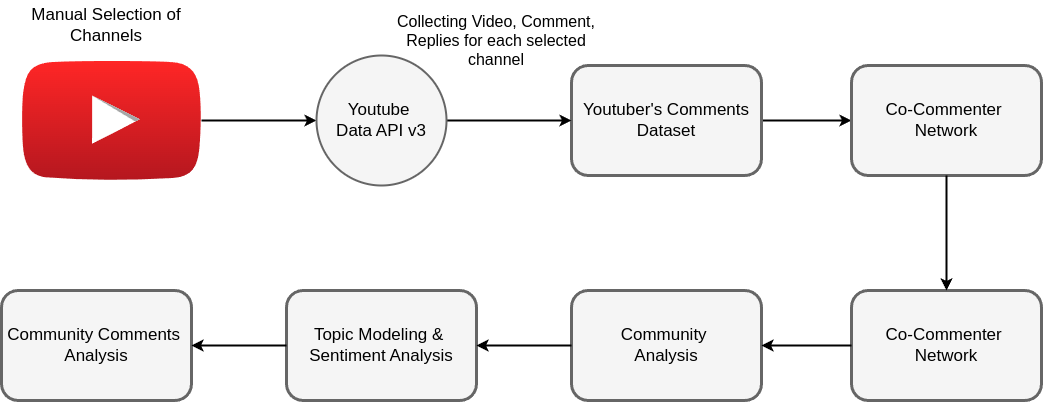
\includegraphics[keepaspectratio,width=0.9\textwidth]{./imgs/tcc_methodology.png}
    \caption[width=\textwidth]{Methodology}
    \label{fig:methodology}
\end{figure*}

\subsection{Data Collection}

Initially, the YouTube Data API v3 was used to gather comprehensive channel metadata for each 
specific YouTuber. Subsequently, we retrieve the IDs and titles of 50 videos from each channel. 
Finally, we construct the YouTuber's comments dataset by aggregating all comments and replies 
associated with each video, as well as the author information and the number of likes of each comment. 
For this, 10 different popular YouTube channels were chosen, with content varying from gaming and 
vlogging, with the number of subscribers ranging from 8 million to 46 million. The number of comments
collected per channel ranges approximately 11,000 to 43,000.


\subsection{Community Analysis}

To analyze the communities that emerge within each YouTuber's comment section, the datasets constructed 
in the previous phase is used to construct the co-commenter networks. Each commenter is connected to
another if they commented on the same video, and the weight of the edge is increased if they commented
on more than one video together. To maintain only the stronger connections, we filtered out co-commenters
who commented on less than 10 videos together, as done by \cite{shajari2023} and \cite{kirdemir2023}. 

To identify the communities of each co-commenter network the Louvain Algorithm was used. This 
algorithm was chosen because of its high efficiency and performance on real-world networks
without ground truth, as shown by \cite{YOU2020104822}.

Following the method developed by \cite{kirdemir2023}, a set of metrics were computed 
for each co-commenter network, including average degree, number of nodes and edges, average coefficient,
modularity, coverage, the number of communities identified with the Louvain Algorithm. Graph clique 
metrics were also computed, including the number of maximal cliques that have at least five members, 
average clique size, median clique size, average degree of clique members, average clustering coefficient
of clique members. To discover the similarities between the chosen channels, these metrics were used
with KMeans and Hierarchical Clustering, along with Principal Component Analysis to reduce the complexity
while maintaining important features.

\subsection{Comments Analysis}

To further understand user behavior, we implement
topic modeling and sentiment analysis. For the topic modeling phase, we employ the BERTopic model 
(\cite{bertopic2022}), while the sentiment analysis is conducted using the multilingual 
XLM-roBERTa-base model(\cite{barbieri-etal-2022-xlm}). 
Initially, the comments are processed and cleaned, masking user handles to preserve anonymity,
removing emojis, links and stop words
Then, topic modeling is utilized to extract themes associated with the communities identified in the 
previous phase. Finally, the sentiment analysis model evaluates the polarity of the content, 
offering deeper insights into the emotional tone of the discussions and facilitating a more 
comprehensive analysis of the communities.

\section{Results}

In this section, the results are shown and analyzed.
Considering that a modularity value above 0.3 is a good indicator of significant
community structures in a network \cite{PhysRevE.70.066111}, The louvain algorithm successfully 
identified significant community structures in all the YouTube creator's co-commenter networks.

The KMeans and Hierarchical Clustering methods were applied with the community metrics described. 
Both methods identified 4 distinct clusters, as can be seen in Figure ~\ref{fig:kmeans_hierarchical}.

\begin{figure*}[ht]
    \centering
    \begin{minipage}{0.44\textwidth}
        \centering
        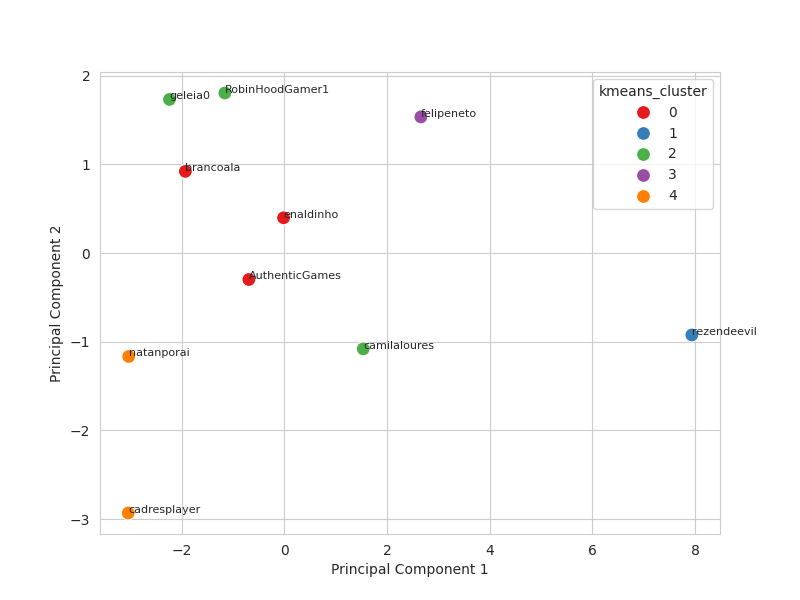
\includegraphics[keepaspectratio,width=\textwidth]{./imgs/KMeans_PCA.png}
    \end{minipage}%
    \hspace{0.0001\textwidth} 
    \begin{minipage}{0.45\textwidth}
        \centering
        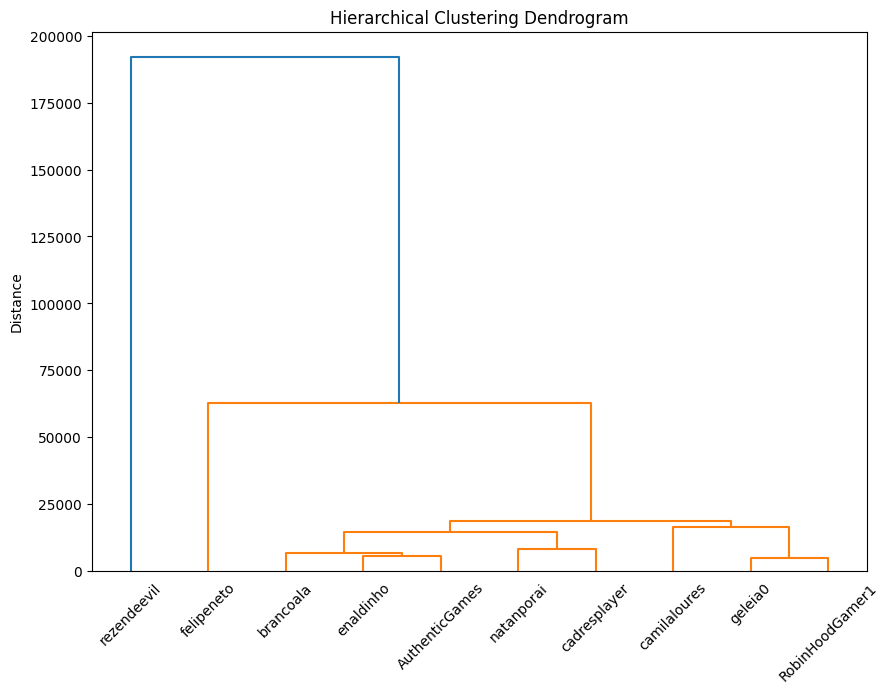
\includegraphics[keepaspectratio,width=\textwidth]{./imgs/Hierarchical_clustering.png}
    \end{minipage}
    % \small % or \footnotesize for even smaller text
    \caption{KMeans and Hierarchical Clustering}
    \label{fig:kmeans_hierarchical}
\end{figure*}


The most distinguishable channels are on clusters 1 (Rezendeevil) and 3 (Felipe Neto). 
Both creators had very large co-commenter networks, with Rezendeevil's network having 13.808 
nodes and 149.033 edges, and Felipe Neto having 24.987 nodes and 125.165 edges.
The creator Rezendeevil, who has the lowest modularity also had the highest 
average degree of 21.5, number of maximal cliques and average clique size.
Similarly, Felipe Neto had a lower modularity score of 0.64, a high number of maximal cliques,
and a high average degree of 10.
This indicates that both creators have high interconnected and engaged communities. The higher average
degree indicates that Rezendeevil's followers are more engaged than Felipe Neto's, while the higher
modularity score shows that Felipe Neto's community structure is more distinct.
This can be seen through Figure~\ref{fig:rezendeevil_comm} and Figure ~\ref{fig:felipeneto_comm}, 
with each community colored.

A per community sentiment analysis showed that most comments on Rezendeevil's videos were labeled as 
positive by the XLM-roBERTa-base model, which is consistent with a highly engaged community of fans.
Most positive comments focus on the video content or specific individuals featured in the video, 
along with compliments directed towards the creator. Through topic analysis, a recurring theme labeled 
"quero" was identified, with comments such as "Eu quero" and "Eu quero muito uma." 
(translated as "I want" or "I really want one").
These comments predominantly come from members of communities 5 and 6. A more detailed investigation 
of the videos receiving these comments may reveal potential signs of direct or implicit advertising 
aimed at children and teenagers.

Unlike the previous creator, Felipe Neto had more negative comments than positive comments. 
By analyzing the polarity per community, it was possible to identify that community 12, 
that has the smallest number of positive comments, is also the community with the highest clustering 
coefficient of approximately 0.23 , lowest conductance of approximately 0.06 and highest density 
of 0.21. This can be an indicative of a close-knit organized community that frequently comment on the 
same content spreading negative and hateful comments. 
Topic Modeling also shows recurring themes labeled "Brasil", "Hipocrisia" 
("Hypocrisy"), "Dinheiro, Pobres" ("Money, Poor"), with comments such as 
"é tanta burrice por metro quadrado é um absurdo como tem gente que acredita nestas hipocrisias" 
("it's such stupidity per square meter, it's absurd how many people believe in these hypocrisies."),
"Esse Felipe merda é uma das desgracas que so existe aqui no Brasil, ..." 
("This Felipe piece of trash is one of the disasters that only exists here in Brazil, ..."). 
The other communities had lower densities, lower average clustering coefficients and higher values 
of conductance, with a wider variety of topics and higher number of positive comments. 


\begin{figure*}[t!]
    \centering
    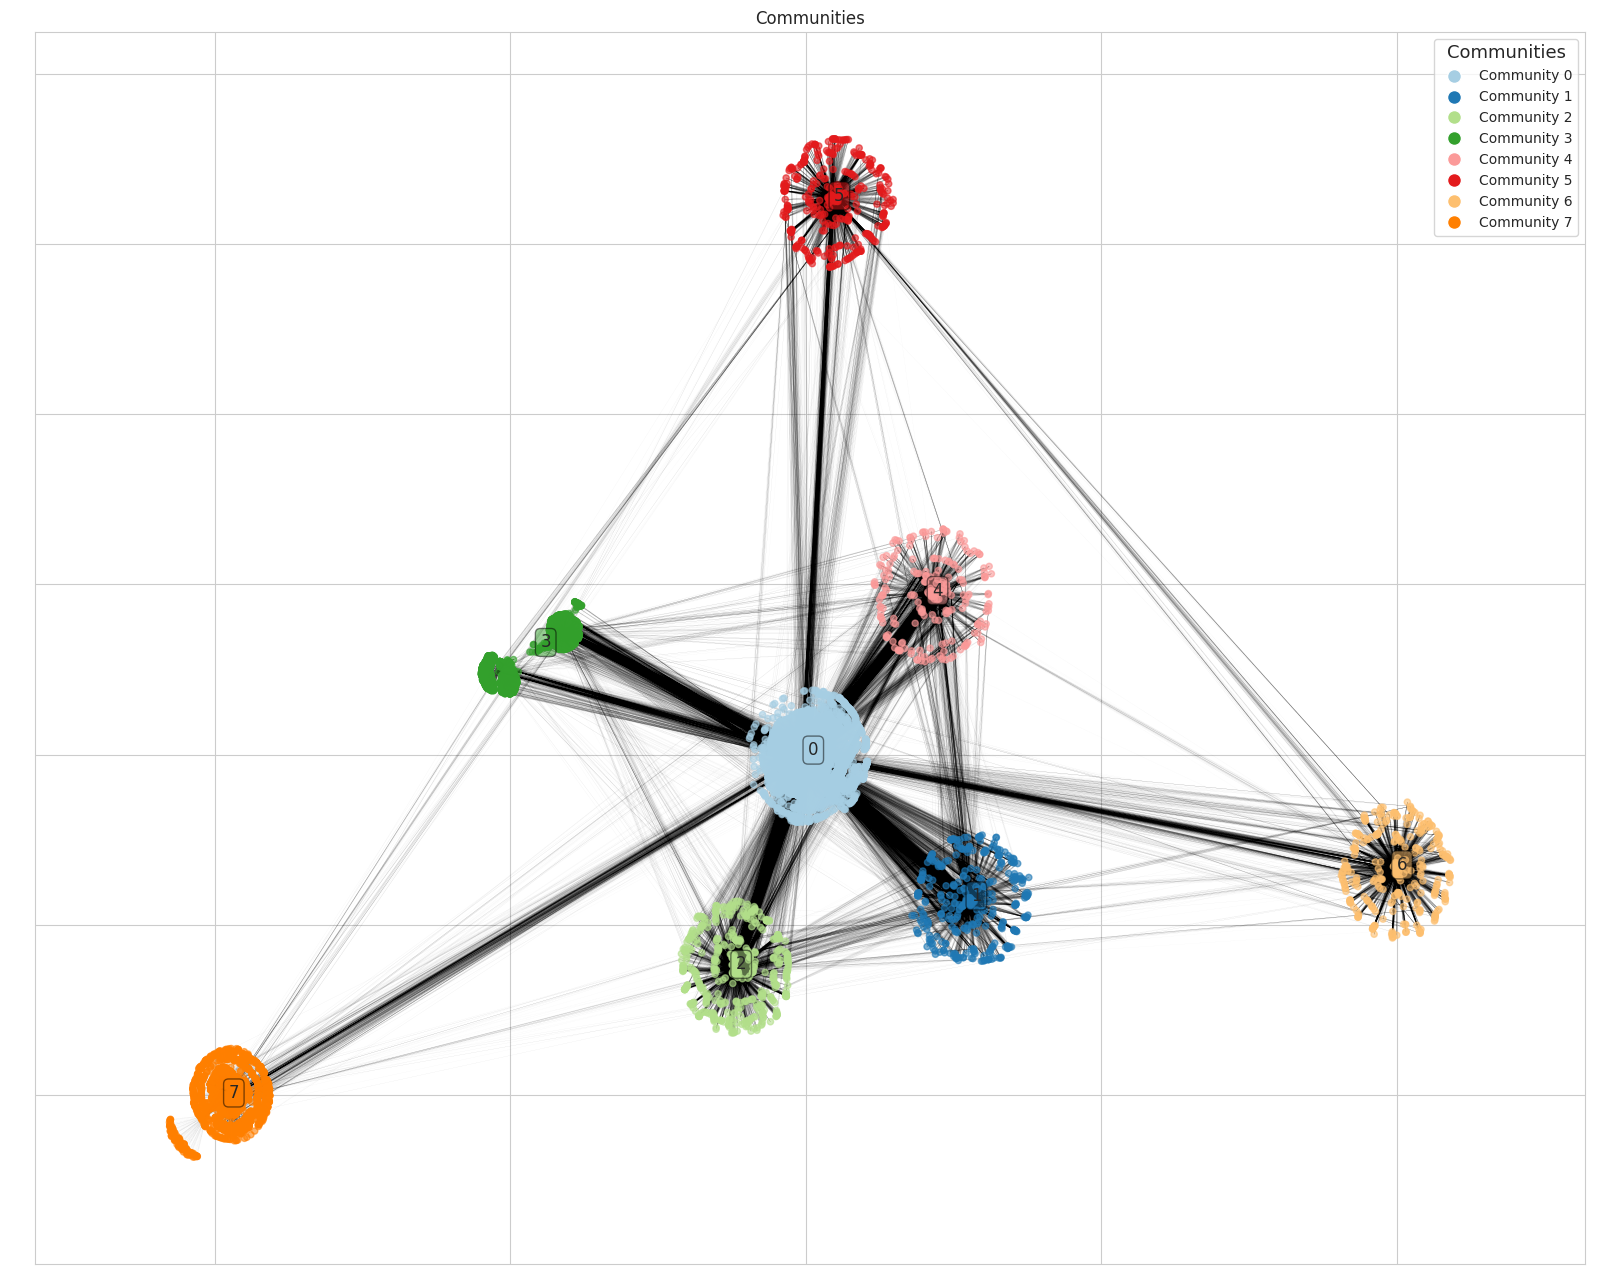
\includegraphics[keepaspectratio,width=0.9\textwidth]{./imgs/rezendeevil/communities.png}
    \caption[width=\textwidth]{Rezendeevil's Communities}
    \label{fig:rezendeevil_comm}
\end{figure*}

\begin{figure*}[t!]
    \centering
    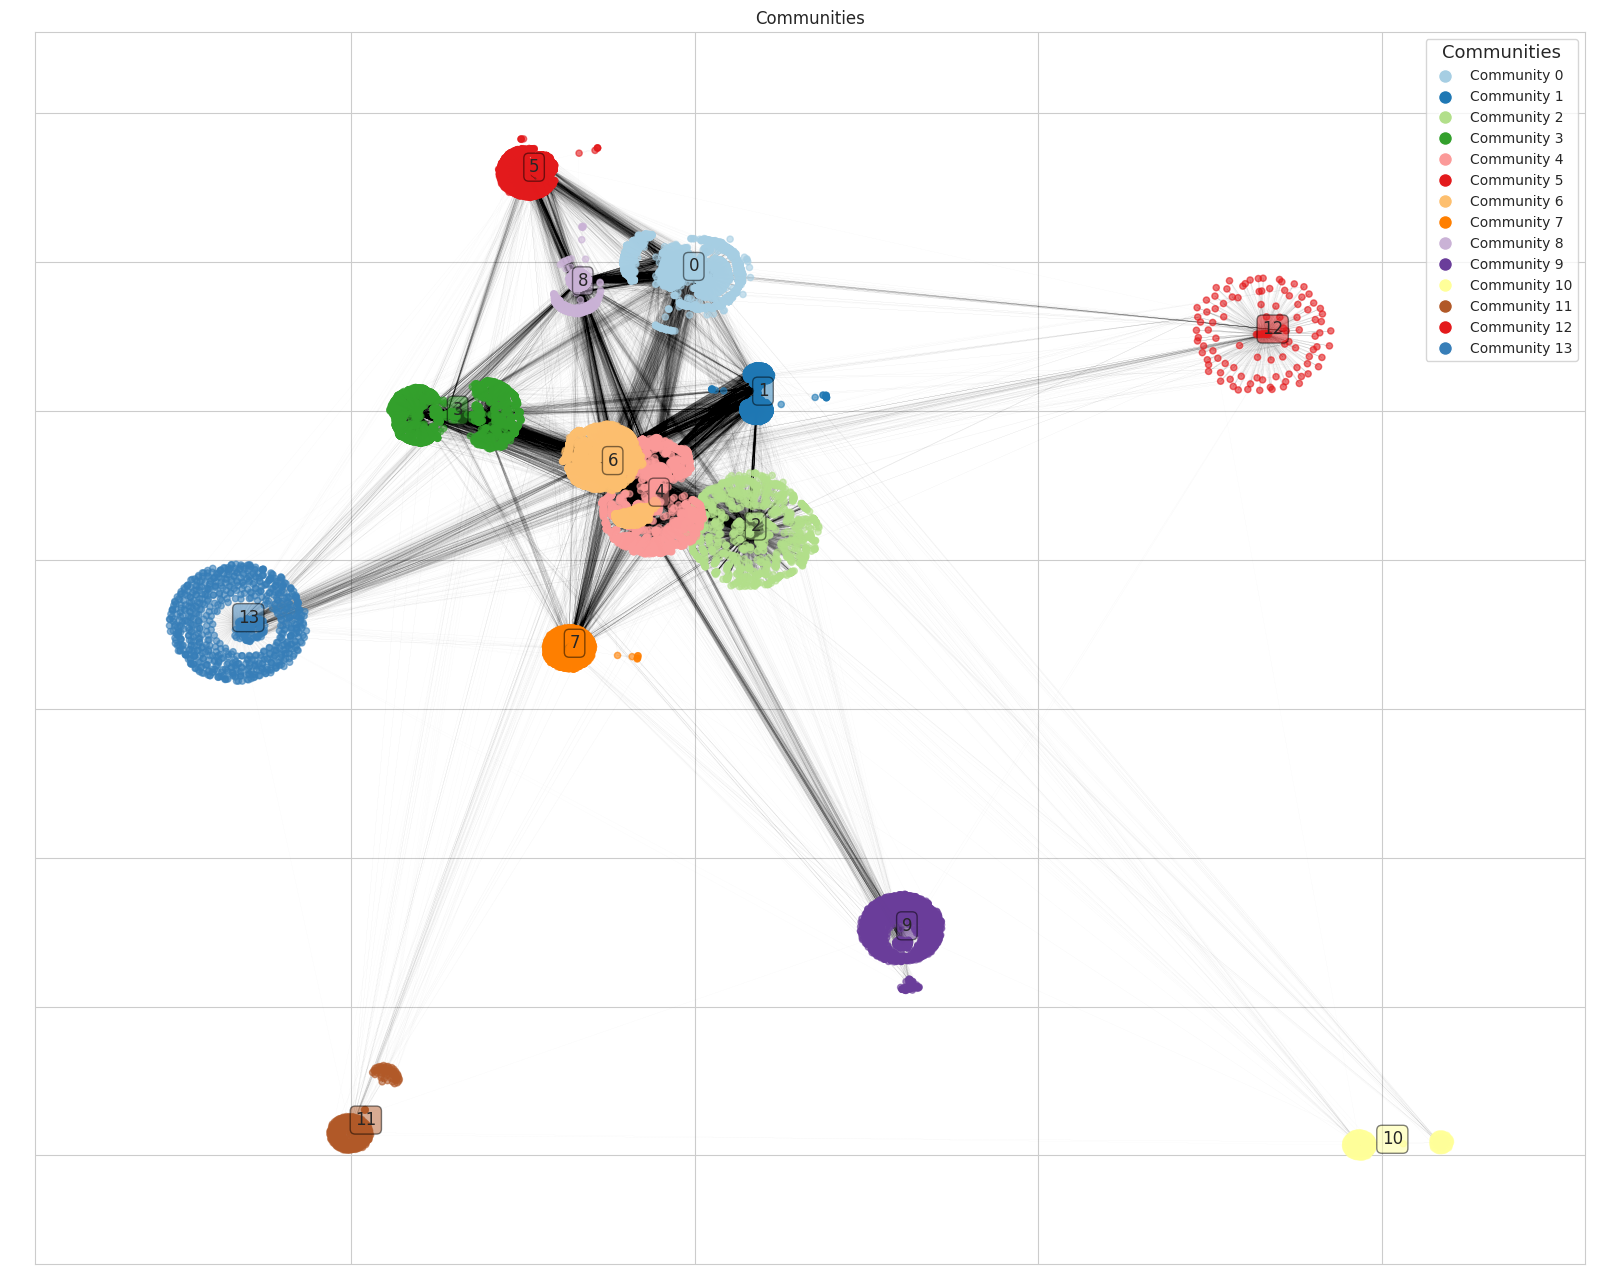
\includegraphics[keepaspectratio,width=0.9\textwidth]{./imgs/felipeneto/communities.png}
    \caption[width=\textwidth]{Felipe Neto's Communities}
    \label{fig:felipeneto_comm}
\end{figure*}


\bibliographystyle{sbc}
\bibliography{sbc-template}

\end{document}
